\documentclass[journal]{IEEEtran}
%\usepackage{lineno}
%\linenumbers
%\usepackage{cite}
\usepackage{amsmath}
\usepackage{siunitx}
\usepackage{hyperref}
\usepackage{amsfonts}

\ifCLASSINFOpdf   
   \usepackage[pdftex]{graphicx}     
   % declare the path(s) where your graphic files are       
   \graphicspath{{../pdf/}{../jpeg/}{./image/}}    
   % and their extensions so you won't have to specify these with    
   % every instance of \includegraphics      
   \DeclareGraphicsExtensions{.pdf,.jpeg,.png,.jpg}   
 \else   
   % or other class option (dvipsone, dvipdf, if not using dvips). graphicx     
   % will default to the driver specified in the system graphics.cfg if no   % driver is specified.    
   \usepackage[dvips]{graphicx}   
   % declare the path(s) where your graphic files are     
   \graphicspath{{../eps/}}    
  % and their extensions so you won't have to specify these with   
  % every instance of \includegraphics    
  % \DeclareGraphicsExtensions{.eps}   
\fi

\hyphenation{}


\begin{document}
\title{828Q - Title}
\author{Jacob Bunker, Thomas Perrin, Jack Sturtevant}
%\markboth{Project description}%
%{}


% make the title area
\maketitle

%\IEEEpeerreviewmaketitle

\section{Abstract}
    Past studies have shown success using evolutionary strategies to train neural networks. This report investigates how evolutionary strategies can be used to train neural networks dedicated to solving sub tasks, and a 'commander' neural network that selects which
    subtasks to execute inorder to complete a larger, more complex task. The scenario the neural networks are being optimized to solve is a two-dimensional 'war-game' simulation in which networks are competign to locate and 'eliminate' one another. Networks that 'survive'
    each scenario are determined to be more fit, and are selected as parents for the next generations in the evolutionary strategies algorithm. Optimizations for training the neural networks are made to create a tradeoff between the simplicity of feed-forward neural
    networks, and the complexity of full connected neural networks. This involves having mini-networks inside which all nodes are fully connected, and sparse connections between nodes in different mini-networks. 

\section{Literature Review}
    Neural Networks have proven their ability to solve complex games with large search spaces. These Networks have been used to solve games as complex as Go, which has an enormous search space. This game has an optimal value function, 
    but the search space has a search tree of size $b^d$. For Go, this search space is defined with ($b \approx 250, d \approx 150)^1$. This makes exhuastive search infeasible \textsuperscript{2,3}, so the search space must be reduced. In order to solve this complex problem
    two separate neural networks are used, a 'value network' for evaluating the board, and a 'policy network' for generating moves\textsuperscript{4}. These networks are trained via a combination of supervised learning from data about games played by exper Go players,
    and reinforcement learning through self-play\textsuperscript{4}.

    Further extensions for training neural networks involve using Evolutionary Strategies\textsuperscript{5}. Historically, reinforcement learning has been used to train neural networks for complex tasks in gaming\textsuperscript{6}. However, evolutionary Strategies
    have demonstrated an alternate solution to reinforcement learning with comparable results, while reducing the complexity and training time required for models\textsuperscript{5}. Evolutionary Strategies does not require backpropagation, is highly parallelizable, is more robust, 
    has structure exploration, and performs better when actions have lasting effects\textsuperscript{5}. Experimental results have demonstrated that neural networks can acheive comparable results to those of reinforcement learning in a time of one hour, compared to a training
    time of one day for reinforcement learning. Evolutionary strategies does have tradeoffs of lower model performance, though the difference is neglible, and reduced efficiency when compared to reinforcement learning\textsuperscript{5}.

    The use of neural networks for agent navigation has been studied extensively\textsuperscript{7,8}. Much of the exploration in this space has been for autonomous robot navigation. These networks are based on standard feed-forward neural networks, which have
    demonstrated shortcomings when solving complex 2D environment. However, recurrent neural networks have shown an ability to solve 2D navigational problems that cononical neural networks have struggled with\textsuperscript{9,10}. Using simultaneous recurrent network
    which draw similarities to the hippocampus, difficult 2D navigation problems like maze navigation have been solved\textsuperscript{9}.

    Extensions to conventional neural networks that reduce the number of internal connections, and modify how they interact, have demonstrated equivalent functionality with reduced training times\textsuperscript{11,12}. Recurrent neural networks based on 
    Nonlinear AutoRegressive models with eXogenous Inputs (NARX models) have demonstrated an ability to limit the amount of feedback within a network without experiencing computational loss\textsuperscript{11}. These networks only limit feedback to so it only comes 
    from output neurons, and not from hidden layers. These demonstrated that a significant reduction in feedback from conventional recurrent neural networks can be made without compromising the computation power of the model. Further studies show that a dynamical model 
    of sensors can be accurately developed using recurrent neural networks as nodes. Essenatial, this model creates a larger network with internal nodes which are in turn recurrent neural network\textsuperscript{12}. These nodes then share information with a confidence factor, which can
    be viewed as a logical equivalent to connection weights in a neural network. This model is able to accurately describe a dynamical model, and demonstrated effectiveness when compared to conventional methods like the Kalman filter method\textsuperscript{12}. 

\section{Methods}
    The goal of this research is to determine if a recurrent neural network with a modified topology can be evolved to 
    compete sucessfully in simulated war game. The topology of these networks are modified so have sections of a network similar
    to the sections in a brain. Furthermore, the network is evolved using evolutionary strategies. Our goal is to evaluate the 
    clustering method against the fully connected method in order to see if the clustering method, which has far less
    memory required per neuron, can produce the same or better results

    \subsection{War Game}
    The scenario in which the neural networks are being trained is a simple simulated war game. In this game, the networks control an agent
    with the ability to move, look, and shoot. Each game consists of two teams of equal size, consisting of 1 or more agents, each controlled by its own network.
    These teams have the goal of finding and eliminating all agents on the other teams. Meanwhile, the agents are trying to survive, and keep their other teammates alive.
    These agents shoot lazers that will hit the first agent or obstacle in the lazer's path. These lazers will always do the same amount of damage to an agent they hit.

    \subsection{Clustering Method}
    The topology of the networks used in this study are different from a normal recurrent neural network. 
    Our inspiration comes from the brain which is roughly separated into modular ‘regions’ with connections between them.
    Instead of being fully
    connected between all nodes, the network consists of clusters of fully connected neurons. The size of each cluster is $N^2$,
    forming an $NxN$ square of fully connected neurons. These clusters  Each of these clusters are their own node within a graph network. 
    To simulate how brain sections which are close in distance tend to have many connections,
    the edge neurons of a given cluster are connected to the edge neurons of the adjacent cluster. Additionally, to maintain 
    that sections of the brain which are far apart have sparse connections, each neuron will have one random connection to 
    another neuron in a different cluster, which need not be adjacent. This allows our network to have connections between all
    neurons, while still significantly reducing memory use. 

    \begin{figure}[h]
      \centering
      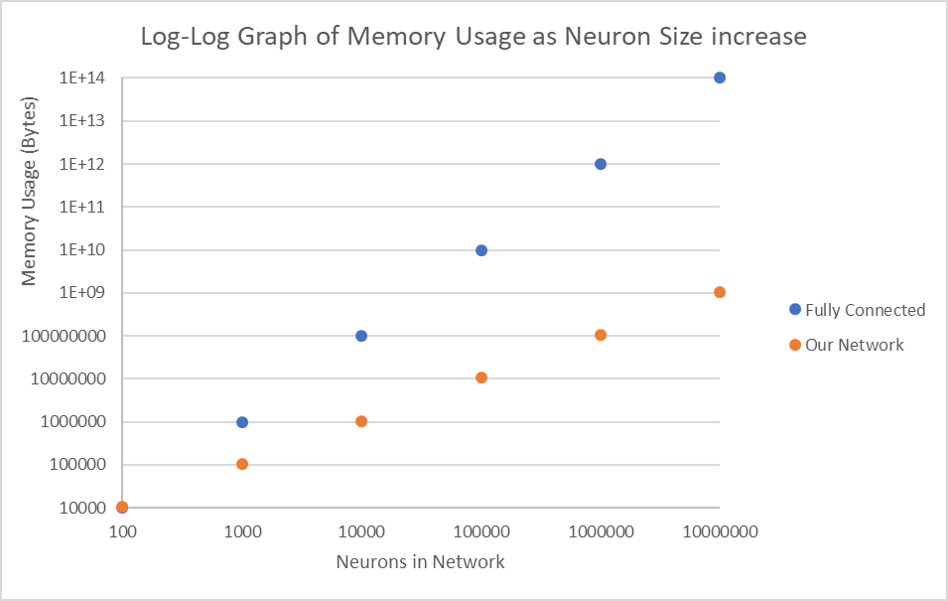
\includegraphics[width=0.25\textwidth,natwidth=300,natheight=200]{fig/828.png}
      \caption{Animal call signal in time domain, taken at a sampling frequency of $5\si{\kilo\hertz}$.}
      \label{fig:call}
  \end{figure}
  

    \subsection{Evolutionary Strategies}
    These networks use evolutionary strategies for training methods. The fitness of a given network is determined by its performance
    in the war simulation. Specifically, if an agent hits an enemy agent with their lazer, their fitness will increase by one. Likewise,
    and agent that is shot by another agent will have their fitness decrease by one. Elitism is used across generations, ensuring the 
    best performing agent in a game is passed to the next generation. 

    \textbf{FILL THIS IN}. Mutations are made using the $1/5th$ rule, using $c=\textbf{FILL THIS IN}$.
    Mutations in these networks can be any of the following: modify weights of a connection, changing which nodes have connections,
    adding or removing a neuron. Additionally, crossover is \textbf{FILL THIS IN}. The selection strategy for developing new 
    prodigy is \textbf{FILL THIS IN}. Finally, elitism is used to ensure propogation of strong networks. 

\section{Sources}
1. Allis, L. V. Searching for Solutions in Games and Artificial Intelligence. PhD thesis, Univ. Limburg, Maastricht, The Netherlands (1994).\\
2. van den Herik, H., Uiterwijk, J. W. and van Rijswijck, J. Games solved: now and in the future. Artif. Intell. 134, 277–311 (2002).\\
3. Schaeffer, J. The games computers (and people) play. Advances in Computers
52, 189–266 (2000)\\
4. Silver, D., Huang A., Maddison, C. J., Guez, A., Sifre, L., van den Driessche, G., Schrittwieser, J., Antonoglou, I., Panneershelvam, V., Lanctot, M., Dieleman, Grewe, D., Nham, J., Kalchbrenner N., Sutskever, I., Lillicrap, T., Leach, M., Kavukcuoglu, K., 
Graepel, T. and Hassabis, D. Mastering the game of Go with deep neural networks and tree search (2016). \\
5. Karpathy, A., Salimans, T., Ho, J., Chen, P., Sutskever, I., Schulman J., Brockman G. and Sidor S. Evolution Strategies as a Scalable Alternative to Reinforcement Learning\\
6. Mnih, V., Kavukcuoglu, K., Silver, D., Graves, A., Antonoglou, I., Wierstra, D., and Riedmiller, M. Playing Atari with Deep Reinforcement Learning (2013)\\
7. Pomerleau, D. A. Neural Network Based Autonomous Navigation. The Kluwer International Series in Engineering and Computer Science (1990)\\
8. Pomerleau, D. A. Efficient Training of Artificial Neural Networks for Autonomous Navigation. (1991)\\
9. Werbos, P. J., Pang, X. Generalized maze navigation: SRN critics solve what feedforward or Hebbian nets cannot. IEEE International Conference on Systems, Man and Cybernetics. Information Intelligence and Systems (1996)\\
10. Ilin, R., Kozma, R., Werbos, P. J. Efficient Learning in Cellular Simultaneous Recurrent Neural Networks - The Case of Maze Navigation Problem. IEEE International Symposium on Approximate Dynamic Programming and Reinforcement Learning (2007)\\
11. Siegelmann, H. T., Horne B. G., Giles, C. L. Computational capabilities of recurrent NARX neural networks. IEEE Transactions on Systems, Man, and Cybernetics. 1997\\
12. Moustapha, A. I., Selmic, R. R. Wireless Sensor Network Modeling Using Modified Recurrent Neural Networks: Application to Fault Detection. IEEE Transactions on Instrumentation and Measurement. 2008\\

\end{document}


